\documentclass[11pt,a4paper]{report}

\usepackage{url}
\usepackage{listings}
\usepackage{graphicx}
\usepackage{hyperref}
\hypersetup{
    colorlinks=true,
    linkcolor=blue,
    filecolor=magenta,      
    urlcolor=cyan,
}

\title{Fi-Pi Software Manual }
\author{e-Yantra summer internship 2017}
\date{July 5,2017}

\begin{document}
	\maketitle
	\newpage
	\tableofcontents{}
	\newpage
	
	\chapter{Installation of an Operating System on Raspberry Pi}
	\section{Objective}
	\begin{flushleft}
	 This chapter will help a Windows or a Linux user to install an operating system on Raspberry Pi successfully.
	\end{flushleft}
	\section{Prerequisites}
	\begin{itemize}
		\item An idea about Windows or Linux operating system and their features.
	\end{itemize}
	\section{Hardware Requirement}
	\begin{enumerate}
		\item Raspberry Pi (I will be using Version 2 Model-B+)
		\item Adapter (To power up an R-pi)
		\item SD card reader
		\item PC (either Linux or Windows machine)
	\end{enumerate}
	\section{Software Requirement}
	\begin{enumerate}
		\item Winrar or any other zipping software 
		\item Utorrent or any suitable downloading platform	
		\item win32DiskManager
		\item Memoy card formatter 
	\end{enumerate}
	\newpage
	\section{Theory and Description}
	\begin{flushleft}
	The Raspberry Pi is a series of small single-board computers developed in the United Kingdom by the Raspberry Pi Foundation.Raspberry Pi is a low cost, credit-card sized computer that plugs into a computer monitor or TV, and uses a standard keyboard and mouse. It is a capable little device that enables people of all ages to explore computing, and to learn how to program in languages like Scratch and Python.The Raspberry Pi 2 uses a Broadcom BCM2836 SoC with a 900 MHz 32-bit quad-core ARM Cortex-A7 processor, with 256 KB shared L2 cache It’s capable of doing everything you’d expect a desktop computer to do, from browsing the internet and playing high-definition video, to making spreadsheets, word-processing, and playing games.
	\end{flushleft}
	\section{A comparison between different models and versions of Raspberry pi}
\resizebox{\textwidth}{!}{	\begin{tabular}{ | p{1in} | p{1in} | p{1in} | p{1in } | p{1in} | p{1in} |}	
	\hline
	Parameter & Model A & Model A+ & Model B & Model B+ & Generation 2 Model B \\
   	\hline	
	\textbf{Target price(in US dollars):} & 25 & 20 & 35 & 25 & 35 \\
	\hline	
	\textbf{SoC:} & Broadcom BCM2835 (CPU, GPU, DSP, SDRAM, one USB port) & Broadcom BCM2835 (CPU, GPU, DSP, SDRAM, one USB port) & Broadcom BCM2835 (CPU, GPU, DSP, SDRAM, one USB port) & Broadcom BCM2835 (CPU, GPU, DSP, SDRAM, one USB port) & Broadcom BCM2836 (CPU, GPU, DSP, SDRAM, one USB port) \\
	\hline 
	\textbf{CPU:} & 700 MHz single-core ARM1176JZF-S & 700 MHz single-core ARM1176JZF-S & 700 MHz single-core ARM1176JZF-S & 700 MHz single-core ARM1176JZF-S & 900 MHz quad-core ARM Cortex-A7 \\
	\hline	
	\textbf{Memory (SDRAM):} & 256 MB (shared with GPU)	512 MB & 256 MB (shared with GPU) & 512 MB (shared with GPU) & 512 MB (shared with GPU) & 1 GB (shared with GPU) \\
	\hline 
	\textbf{USB 2.0 ports:} & 1 (direct from BCM2835 chip) & 1 (direct from BCM2835 chip) & 2 (via the on-board 3-port USB hub)[38] & 4 (via the on-board 5-port USB hub) & 4 (via the on-board 5-port USB hub) \\
	\hline 
	\textbf{On-board storage:} & SD / MMC / SDIO card slot (3.3 V with card power only) & MicroSD slot[32] & SD / MMC / SDIO card slot & MicroSD slot & MicroSD slot \\
	\hline
	\textbf{On-board network:} & None & None & 10/100 Mbit/s Ethernet (8P8C) USB adapter on the third/fifth port of the USB hub (SMSC lan9514-jzx) & 10/100 Mbit/s Ethernet (8P8C) USB adapter on the third/fifth port of the USB hub (SMSC lan9514-jzx) & 10/100 Mbit/s Ethernet (8P8C) USB adapter on the third/fifth port of the USB hub (SMSC lan9514-jzx) \\
	\hline 
	\textbf{Low-level peripherals:} & 8× GPIO & 17× GPIO plus the same specific functions, and HAT ID bus & 8× GPIO  & 17× GPIO  & 17× GPIO \\
	\hline
	\textbf{Power ratings:} & 300 mA (1.5 W) & 200 mA (1 W) &	700 mA (3.5 W) & 600 mA (3.0 W) & 800 mA(4.0 W) \\
	\hline 
	\end{tabular}}
	\centering
	\newpage
	\flushleft
	\section{Experiment}
	
	Instructions for installing operating system in Raspberry Pi:
	
	Download Raspbian software from raspberry pi website. It should be available in the form of a zip file. Download it from the following link: \url{https://www.raspberrypi.org/downloads/} Also download win32DiskManager from the following link:\url{http://sourceforge.net/projects/win32diskimager/} and memorycard formatter (SD Formatter) from :-\url{https://www.sdcard.org/downloads/formatter_4/eula_windows/}then install it.
	
	\vspace{0.5cm}
	A windows user should follow these steps:
	\begin{itemize}
		\item Insert an sd card(4GB or greater size) into the laptop in the memory card slot if available or use a memory card reader.First format the complete memory card using SD Formatter software downloaded from the above link then Run win32DiskImager and choose the Raspbian image and select the drive corresponding to your sd card.
		\item Click "Write" to copy the files of the image on to the sd card.
		\item Eject SD card and insert it into the sd card slot of the Raspberry Pi.
	\end{itemize}
	
	A Linux user should follow these steps:
		\begin{itemize}
			\item Insert an sd card(4GB or greater size) into the laptop in the memory card slot if available or use a memory card reader.
			\item Run df -h to see what devices are currently mounted. The new device that has appeared is your SD card. The left column gives the device name of your SD card; it will be listed as something like /dev/mmcblk0p1 or /dev/sdd1. The last part (p1 or 1 respectively) is the partition number but you want to write to the whole SD card, not just one partition. Therefore you need to remove that part from the name (getting, for example, /dev/mmcblk0 or /dev/sdd) as the device for the whole SD card. Note that the SD card can show up more than once in the output of df; it will do this if you have previously written a Raspberry Pi image to this SD card, because the Raspberry Pi SD images have more than one partition.
			\item Note down your device name. You need to unmount it so that files can't be read or written to the SD card while you are copying over the SD image.
			\item Run umount /dev/sdd1, replacing sdd1 with whatever your SD card's device name is (including the partition number).
			If your SD card shows up more than once in the output of df due to having multiple partitions on the SD card, you should unmount all of these partitions.
			\item In the terminal, write the image to the card with the command below, making sure you replace the input file if= argument with the path to your .img file, and the /dev/sdd in the output file of= argument with the right device name. This is very important, as you will lose all data on the hard drive if you provide the wrong device name. Make sure the device name is the name of the whole SD card as described above, not just a partition of it; for example sdd, not sdds1 or sddp1; or mmcblk0, not mmcblk0p1.
			
			dd bs=4M if=2015-05-05-raspbian-wheezy.img of=/dev/sdd
			
			Please note that block size set to 4M will work most of the time; if not, please try 1M, although this will take considerably longer.
			
			Also note that if you are not logged in as root you will need to prefix this with sudo.
			\item The dd command does not give any information of its progress and so may appear to have frozen; it could take more than five minutes to finish writing to the card. If your card reader has an LED it may blink during the write process. To see the progress of the copy operation you can run pkill -USR1 -n -x dd in another terminal, prefixed with sudo if you are not logged in as root. The progress will be displayed in the original window and not the window with the pkill command; it may not display immediately, due to buffering.
			
			Instead of dd you can use dcfldd; it will give a progress report about how much has been written.
			
			You can check what's written to the SD card by dd-ing from the card back to another image on your hard disk, truncating the new image to the same size as the original, and then running diff (or md5sum) on those two images.
			
			\item The SD card might be bigger than the original image, and dd will make a copy of the whole card. We must therefore truncate the new image to the size of the original image. Make sure you replace the input file if= argument with the right device name. diff should report that the files are identical.
			
			dd bs=4M if=/dev/sdd of=from-sd-card.img
			truncate --reference 2015-05-05-raspbian-wheezy.img from-sd-card.img
			diff -s from-sd-card.img 2015-05-05-raspbian-wheezy.img
			\item Run sync; this will ensure the write cache is flushed and that it is safe to unmount your SD card.
			\item Remove the SD card from the card reader and insert it into Raspberry Pi's SD card slot. [1]
		\end{itemize}
		
	After inserting the SD card into Raspberry Pi follow these steps:
	\begin{enumerate}
		\item Connect the keyboard and mouse.Use HDMI cable to connect the board to the VGA monitor
		\item Power on the board and the monitor. You will notice a set of code running on the monitor.
		\item After a while a software configuration tool opens.
		
			\begin{figure}[h!]
				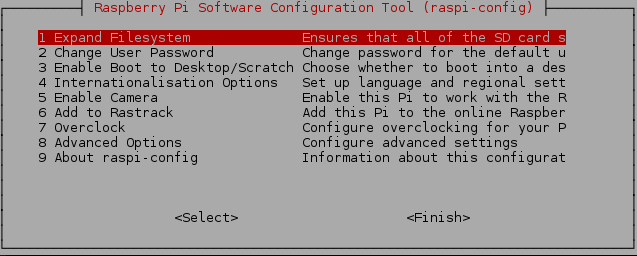
\includegraphics[scale=0.6]{2.PNG}
				\centering
				\caption{}
			\end{figure}
		\item In case the size of the SD card is greater than 4GB you can select the 1st option i.e.Expand file system in the configuration tool as shown above.	
		\item Select the internationalisation options.
			\begin{figure}[h!]
				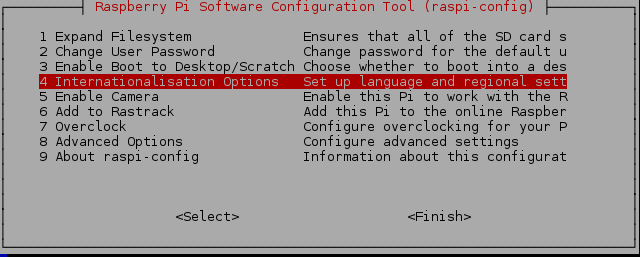
\includegraphics[scale=0.6]{3.PNG}
				\centering
				\caption{}
			\end{figure}
		\item Change the keyboard and language settings as per your choice. Default keyboard will be of UK. Step by step change to US keyboard is as shown:
		\begin{itemize}
		\item First select the option change Keyboard layout and click ok
			\begin{figure}[h!]
				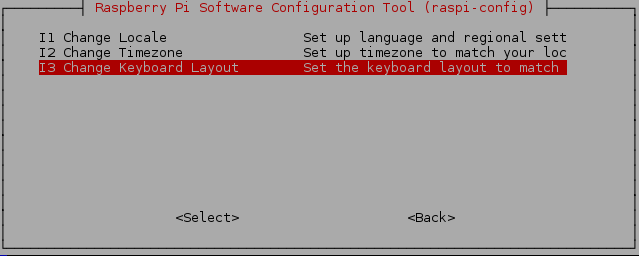
\includegraphics[scale=0.6]{4.PNG}
				\centering
				\caption{}
			\end{figure}
		\newpage
		\item Then select the respective keyboard you are using and if you dont find your kind then select any of the generic types.
			\begin{figure}[h!]
				\includegraphics[width=10cm,height=10cm]{Keyboard-Change2.PNG}
				\centering
				\caption{}
			\end{figure}
		\item Select "English US" which will be available at the top. Then for the rest of the process simply click enter till you reach the main configuration menu.
			\begin{figure}[h!]
				\includegraphics[scale=0.6]{Keyboard-Change3.PNG}
				\centering
				\caption{}	
			\end{figure}
		\end{itemize}
	\newpage
	
	\item Click on finish using the keyboard by using arrow keys and enter key.
	\item Click on "ok" when prompted for reboot.
	\item Upon reboot, enter 'pi' as user id and 'raspberry' as password. Then type 'startx' to enter the graphical interface.
	\item The linux based raspbian interface will be displayed on the monitor. Some of the softwares will be preloaded such as wolfram, python etc.
	\item The command prompt will be the lx terminal.
	\end{enumerate}
	
	With this we end the installation of Raspbian OS in R-Pi.
	
	\vspace{0.4cm} 
	\newpage
	
	\chapter{Establishing Network connection and SSH between pc and Raspberry pi }
	\section{Objective}\
	\begin{flushleft}
	this chapter focuses on learning how to establish a network connection in an R-Pi and how to connect a PC to a Raspberry Pi using SSH connection(i.e. remote control).
	
	\section{Prerequisites}
	One should be aware of :
	\begin{itemize}
		\item Basic terminal commands.
		\item The ssid and password of a wireless network to which an R-Pi has to be connected.
	\end{itemize}
	
	\section{Hardware Requirement}
	\begin{enumerate}
		\item Raspberry Pi (I will be using Version 2 Model B+)
		\item Monitor,HDMI cable,Keyboard,Mouse (This an optional mode of connecting an R-Pi.
		\item Wireless adapter
		\item Power adapter
		\item PC(either Windows or Linux)
	\end{enumerate}
		
	\section{Software Requirement}
	MobaXterm(for Windows user)
	
	\newpage
	\section{Theory and Description}
	Secure Shell is a program to log into another computer over a network, to execute commands in a remote machine, and to move files from one machine to another. It provides strong authentication and secure communications over insecure channels. It is a replacement for rlogin, rsh, rcp, and rdist.
	SSH protects a network from attacks such as IP spoofing, IP source routing, and DNS spoofing. An attacker who has managed to take over a network can only force ssh to disconnect. He or she cannot play back the traffic or hijack the connection when encryption is enabled.
	When using ssh's slogin (instead of rlogin) the entire login session, including transmission of password, is encrypted; therefore it is almost impossible for an outsider to collect passwords. [2]
	\begin{figure}[h!]
		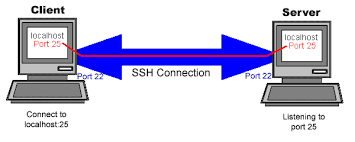
\includegraphics[scale=0.8]{ssh.png}
		\centering
		\caption{[3]}
	\end{figure}
	\textbf{Applications of SSH or OpenSSH protocol}
	\begin{itemize}
		\item For login to a shell on a remote host (replacing Telnet and rlogin)
		\item For executing a single command on a remote host (replacing rsh)
		\item For setting up automatic (passwordless) login to a remote server (for example, using OpenSSH)
		\item Secure file transfer
		\item In combination with rsync to back up, copy and mirror files efficiently and securely
		\item For forwarding or tunneling a port (not to be confused with a VPN, which routes packets between different networks, or bridges two broadcast domains into one).
		\item For using as a full-fledged encrypted VPN. Note that only OpenSSH server and client supports this feature.
		\item For forwarding X from a remote host (possible through multiple intermediate hosts)
		\item For browsing the web through an encrypted proxy connection with SSH clients that support the SOCKS protocol.
		\item For securely mounting a directory on a remote server as a filesystem on a local computer using SSHFS.
		\item For automated remote monitoring and management of servers through one or more of the mechanisms discussed above.
		\item For development on a mobile or embedded device that supports SSH.[1]
	\end{itemize}
	
	\flushleft
	\textbf{MobaXterm}
	\vspace{0.4cm}
	\newline MobaXterm is a tool used for remote computing. In a single Windows application, it provides loads of functions that are tailored for programmers, webmasters, IT administrators and pretty much all users who need to handle their remote jobs in a more simple fashion.It provides all the important remote network tools (SSH, X11, RDP, VNC, FTP, MOSH, ...) and Unix commands (bash, ls, cat, sed, grep, awk, rsync, ...) to Windows desktop, in a single portable exe file which works out of the box. \newline
	
	There are many advantages of having an All-In-One network application for your remote tasks, e.g. when you use SSH to connect to a remote server, a graphical SFTP browser will automatically pop up in order to directly edit your remote files. Your remote applications will also display seamlessly on your Windows desktop using the embedded X server.[4]
		
	\newpage
	
	
	\section{Establishing a network connection}
	Before we can start using a Raspberry Pi remotely we need to configure its network settings.There are two ways to configure network setting:
	\begin{itemize}
		\item One is using DHCP server (wireless connection)
		\item The other one is by assigning a static IP
	\end{itemize}
	\subsection{Network settings configuration using DHCP Server(wireless settings)} 
	\begin{enumerate}
		\item Insert the SD card (with Raspbian OS already written) into the micro SD slot in an R-Pi.
		\item Connect the wireless adapter, keyboard , mouse and monitor (using a HDMI cable) to the Raspberry Pi.
		\item Power on the board and monitor.You will notice a set of code running on the monitor.
		\item Enter the set user name and password and then type \textit{startx} command to launch the GUI.
		\begin{figure}[h!]
			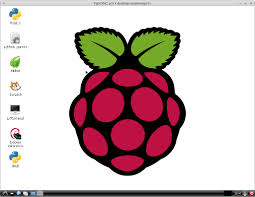
\includegraphics[width=10cm]{r1.jpg}
			\centering
			\caption{}
		\end{figure} 
		\item Click on the icon at the bottom-left on the screen. This is the start icon.
		\item Select LXTerminal option to open a terminal window
		\newpage
		\begin{figure}[h!]
			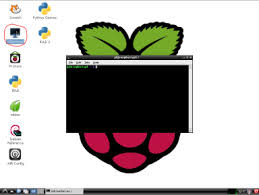
\includegraphics[width=10cm]{lxt.jpg}
			\centering
			\caption{}
		\end{figure}
		\item Some of the previous versions of Raspbian OS do not support wireless module. To know about the version you are using type \textit{uname -a}. To upgrade to the latest one type "sudo apt-get upgrade".
		\item Connect your wireless adapter . To check if its connected type \textit{lsusb}(We used D-link adapter which is highlighted in yellow) 
		\begin{figure}[h!]
			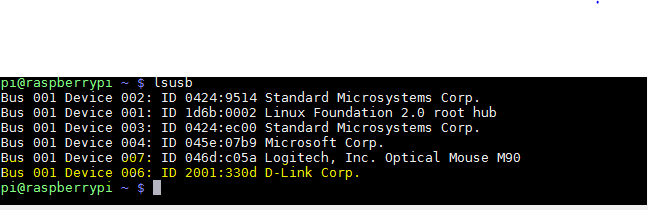
\includegraphics[scale=0.6]{Lsusb.PNG}
			\centering
			\caption{}
		\end{figure}
		\item Now type \textit{sudo nano /etc/network/interfaces} and press enter. You will see the following window:
		\newpage
		\begin{figure}[h!]
			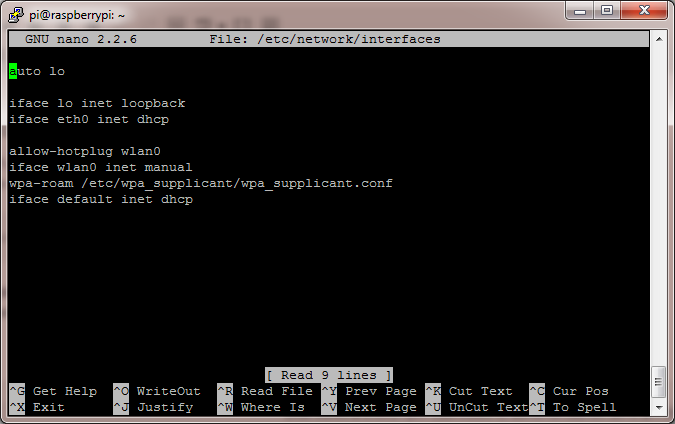
\includegraphics[scale=0.6]{iwifi.png}
			\centering
			\caption{}
		\end{figure}
		\item Change the code by adding the following lines:
		\begin{figure}[h!]
			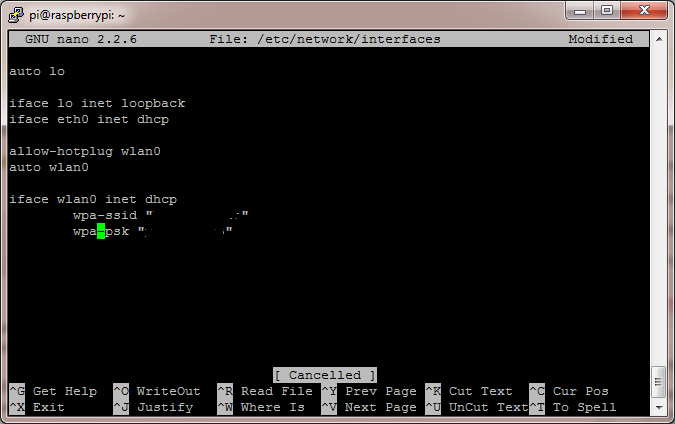
\includegraphics[scale=0.6]{wificon.png}
			\centering
			\caption{}
		\end{figure}
		\item Add in the SSID(username) and Password of your wifi. Then for changes to take effect type \textit{sudo /etc/init.d/networking restart} 
		\item Type \textit{ifconfig} to obtain the IP address of R-Pi etc. It will be under wlan0(written as inet address).
	\end{enumerate}
	
	\newpage
	\subsection{Network settings using static IP method}
	The router normally distributes the dynamic IP addresses but it isn’t guaranteed that it will assign the same IP address every time. This can cause problems if you are trying to connect to your Raspberry Pi remotely. And hence we can assign a static IP. In order to do so follow these steps:
	\begin{enumerate}
		\item Open the LXTerminal and type the following command \newline \textit{cat /etc/network/interfaces}
		\item Before you make changes to the document you should be aware of your current IP address, the broadcast IP and the Mask Use the command \textit{ifconfig} to retrieve this information
		To find your gateway address type the following command: \textit{sudo route \-nee}
		\item In order to edit the interfaces file type \textit{sudo nano /etc/network/interfaces}
		\item Remove the following line \textit{iface eth0 inet dhcp} and add the following:\newline \textit{iface eth0 inet static \newline address 192.168.0.x \newline netmask 255.255.255.0 \newline network 192.168.0.0 \newline broadcast 192.168.0.255 \newline gateway 192.168.0.y }
	    \item Save the file using Ctrl+X, Y.
	    \item For changes to take effect type \textit{sudo /etc/init.d/networking restart} and reboot the system.
    \end{enumerate}
	
	
	\newpage	
	\section{Establishing an SSH connection}
	
	To start using a Raspberry Pi remotely follow these steps:
	\begin{enumerate}
		\item A windows user should download MobaXterm (latest version) using the following link: \url{http://mobaxterm.mobatek.net/}
		\item Run the .exe file and open the application.
		\begin{figure}[h!]
			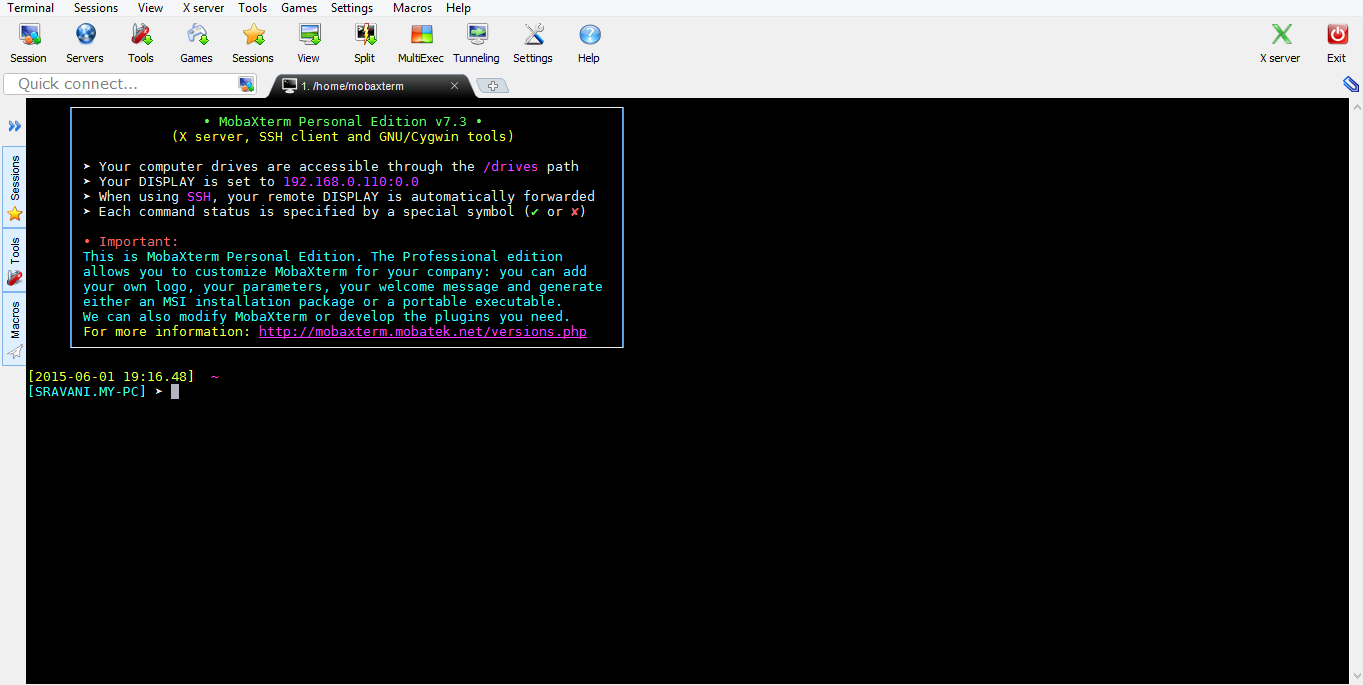
\includegraphics[scale=0.3]{M1.PNG}
			\centering
			\caption{}
		\end{figure}
		\item Then select the session option on the toolbar.
		\begin{figure}[h!]
			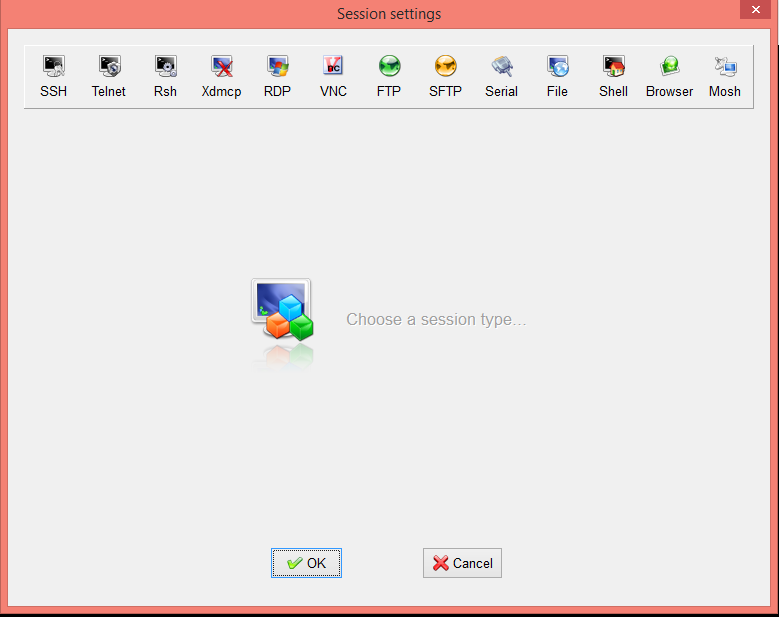
\includegraphics[scale=0.5]{M2.PNG}
			\centering
			\caption{}
		\end{figure}
		\newpage
		\item Click on the SSH option. A settings window opens as shown
		\begin{figure}[h!]
			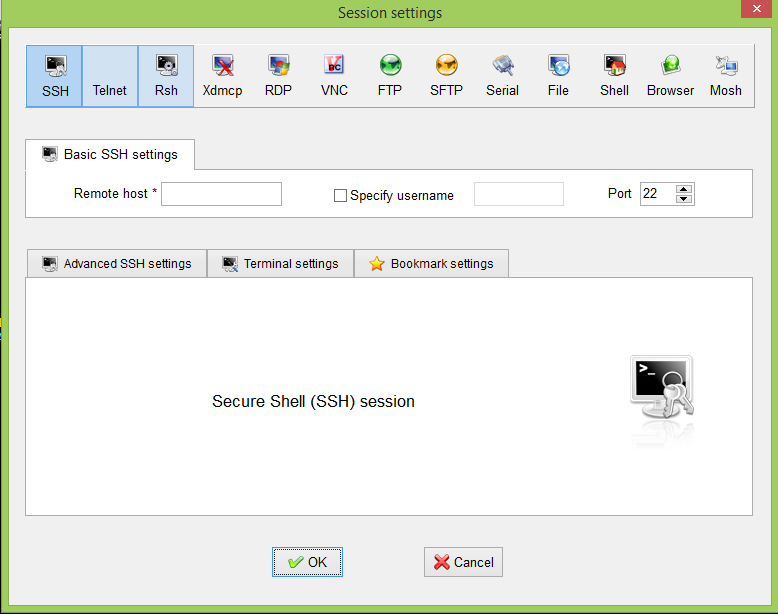
\includegraphics[scale=0.5]{M3.PNG}
			\centering
			\caption{}
		\end{figure}
		\item Enter the IP address of the R-pi in the Remote host field and in the 'Advanced SSH settings' option configure the remote environment either as 'Interactive shell (terminal based)' or as an 'LXDE desktop(GUI based)'and click OK
		\item If you are using the Interactive shell environment login to the R-Pi using the following command: ssh -X pi@192.168.0.4 (IP address of pi) and then enter the login id and password to start using the Pi remotely.
		\item If you are using the LXDE desktop i.e. the GUI environment then use LX terminal icon to start programming the Pi.
		\begin{figure}[h]
			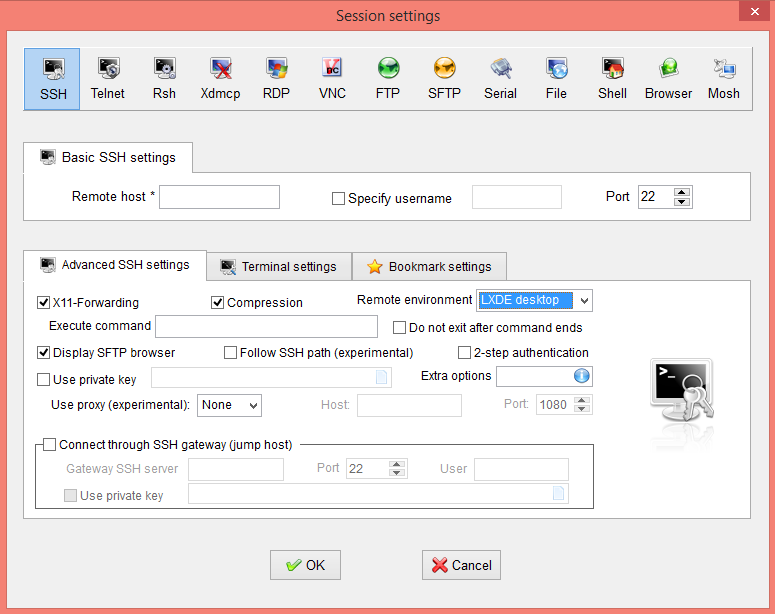
\includegraphics[scale=0.5]{M4.PNG}
			\centering
			\caption{}
		\end{figure}
		\newpage
		\item Also the established session is saved. So the next time you want to access directly click on the R-Pi's address mentioned in the saved session option to start using the Pi remotely.
		\begin{figure}[h!]
			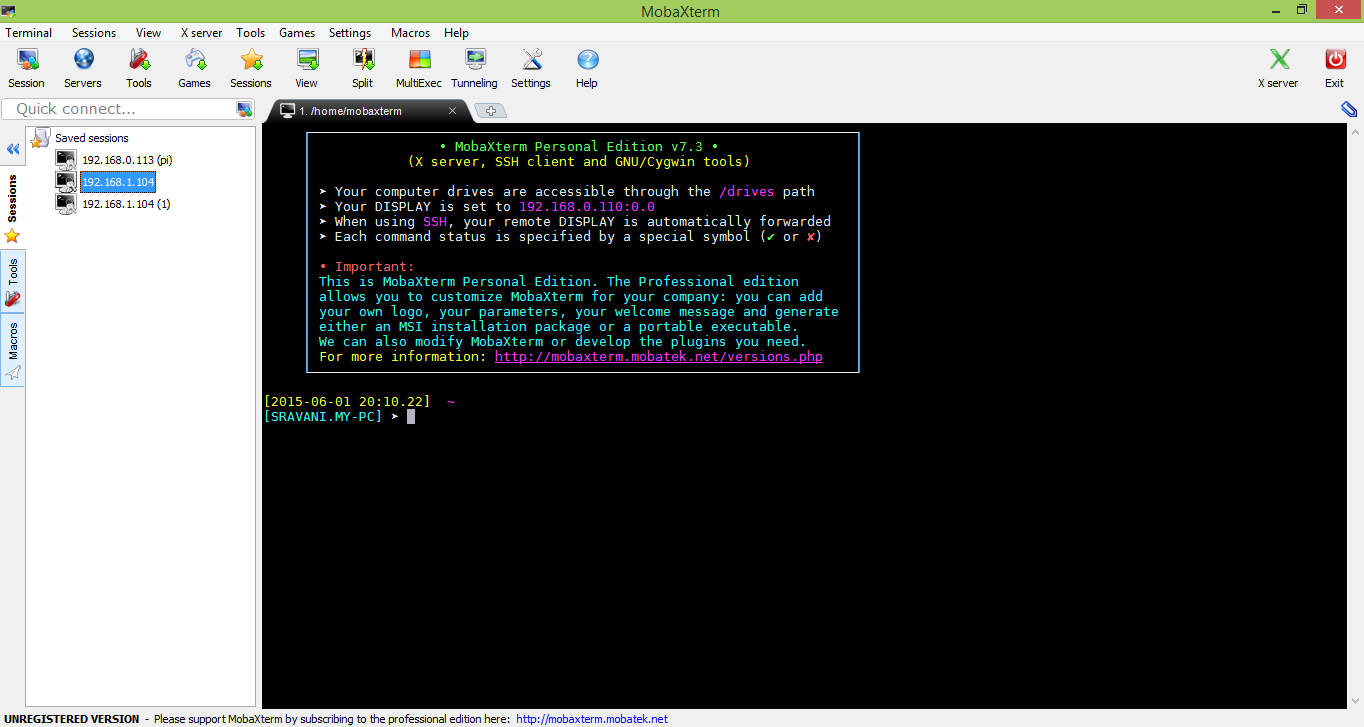
\includegraphics[scale=0.3]{M5.PNG}
			\centering
			\caption{}
		\end{figure}
	\end{enumerate}

	\textbf{Note:} A linux user needn't download any Xterm file. They can directly start accessing the R-Pi using the command: ssh -X pi@192.168.0.4 (IP address of pi) and then entering the login id and password for using the Pi remotely.
	
	\newpage
	
	\chapter{Programming Raspberry-Pi }
	\section{Prerequisites}
	\begin{enumerate}
		\item PyScripter (version 2.7 or above)
		\item Mobaxterm (for windows users)
	\end{enumerate}
	\section{Raspberry-pi J8 Header }
	\textbf{Expansion Header}
	
	The Raspberry Pi 2 Model B+ board contains a single 40-pin expansion header labelled as 'J8' providing access to 26 GPIO pins.
	(Pins 1, 2, 39 and 40 are also labelled below.)
			\begin{figure}[h!]
				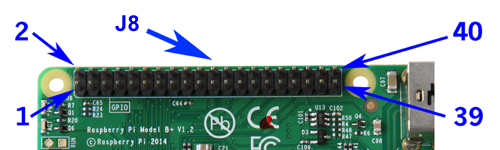
\includegraphics[scale=0.7]{j8h.png}
				\centering
				\caption{[3]}
			\end{figure} 
	
	\newpage
	The diagram below illustrates the pin out diagram of Raspberry Pi 2:
	\begin{figure}[h!]
		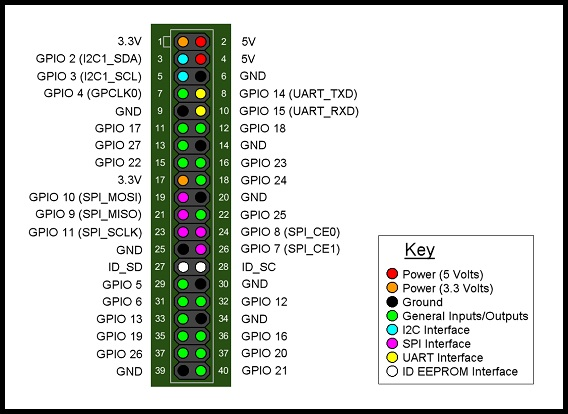
\includegraphics[scale=0.6]{RaspberryPi2_pinout.jpg}
		\centering
		\caption{[4]}
	\end{figure} 
	
	\flushleft
	You must have noticed that the board contains pins named as GPIO (that are used for interfacing input and output devices) and hence in order to refer to the R-Pi pins there exists two modes:
	\begin{enumerate}
		\item \textbf{BCM mode:} Referring the pins with the GPIO number
		\item \textbf{Board mode:} Referring the pins using the IC pin numbers.
	\end{enumerate}
	\section{Different ways of programming}
	Before we write a code to access GPIO pins of the Pi let's understand the different ways to program Pi.
	\begin{enumerate}
		\item GUI based programming using IDLE3. In order to do so follow these steps:
		\begin{itemize}
			\item First, load up IDLE 3 by double-clicking the icon on your LXDE desktop(either on the monitor or using Mobaxterm as explained in the previous tutorial based on establshing a SSH connection).
			\begin{figure}[h!]
				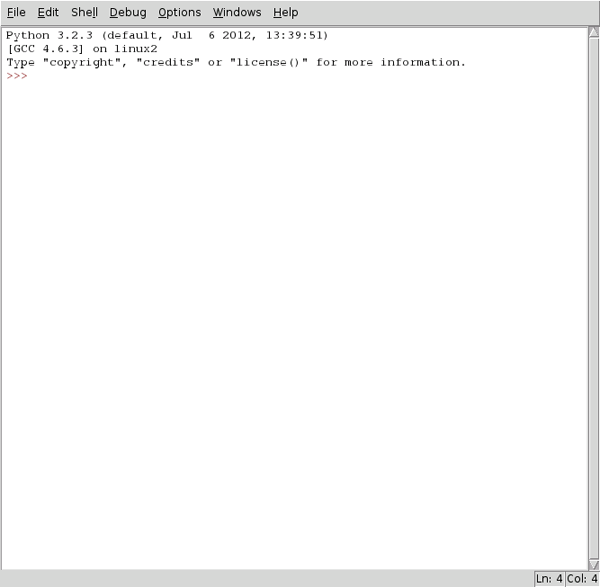
\includegraphics[width=10cm, height=8cm]{idle3.png}
				\centering
				\caption{[1]}
			\end{figure}
			\item Click File,New Window, which will then bring up a new blank window which you can type in.
			\item Now click File,Save As and save your file in the desired folder.
			\item Click Run, and then Run Module or simply press F5.
		\end{itemize}
		\item Terminal based programming:
		\begin{itemize}
			\item Using PyScripter and MobaXterm:
			PyScripter is a free and open-source Python IDE used for programming in Python.In order to download PyScripter use the following link \url{https://code.google.com/p/pyscripter/} (I use version 2.5.3).
			\newline \begin{enumerate}
				\item Open the application. You will see a window like this:
				\begin{figure}[h!]
					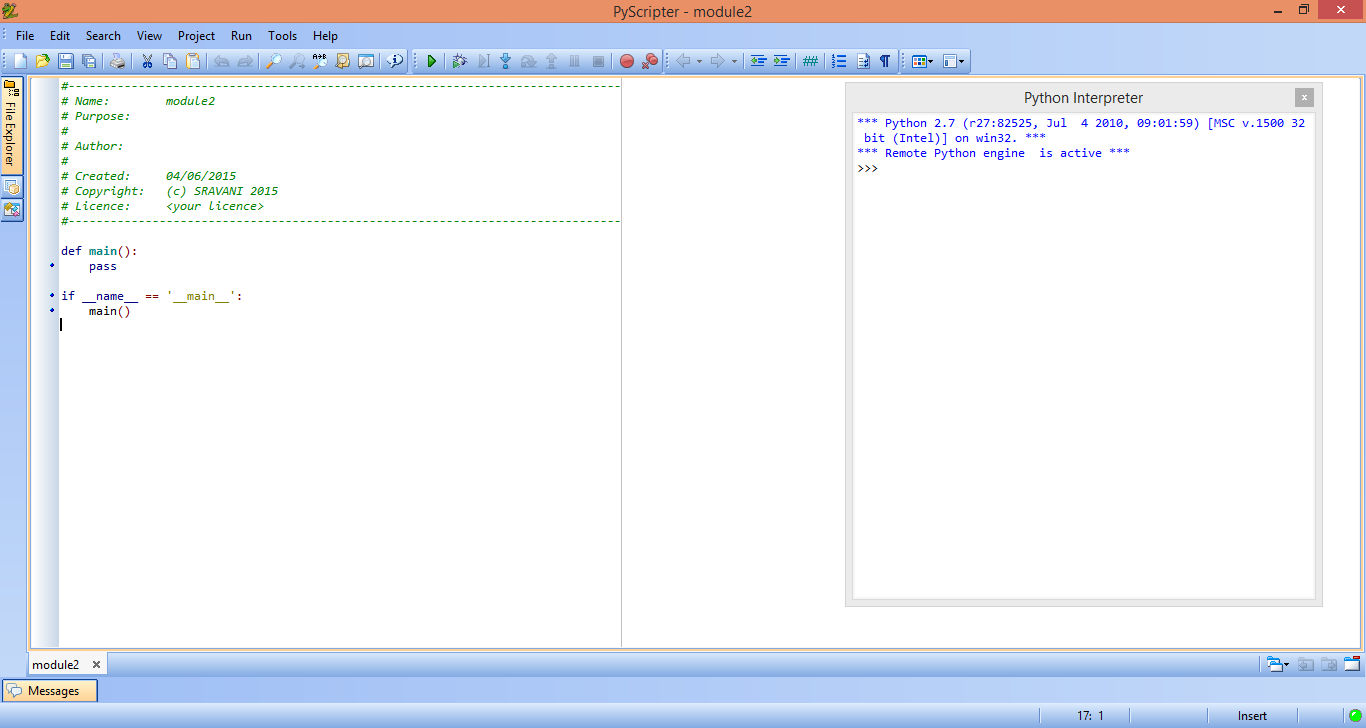
\includegraphics[scale=0.4]{py.png}
					\centering
					\caption{}
				\end{figure}
				\item Delete the text already present and type your program. Once you finish typing the program goto File > Save As and save the program.
				\item Now open MobaXterm. On the left side you can see the files in /home/pi/ directory and you also have some small icons on the toolbar. Click on the icon 'Upload to current folder' as shown:
				\begin{figure}[h!]
					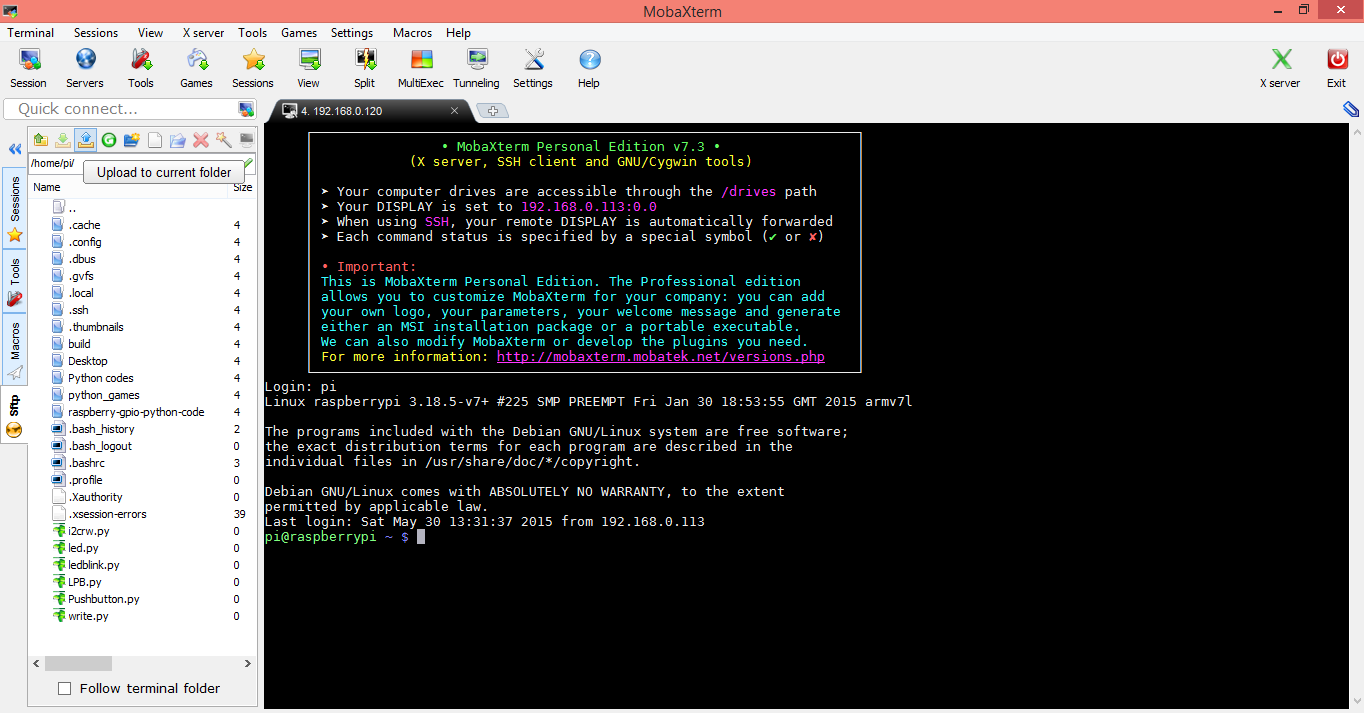
\includegraphics[scale=0.4]{1.png}
					\centering
					\caption{}
				\end{figure}
				\newpage
				\item Upload that file wherein you have written your python program.
				Note: You can either upload your files to the home directory i.e. /home/pi/ or else you can create a new directory using the icons on the toolbar as illustrated before and upload your python file over there.
				\item After you have uploaded the code then type the following command on the terminal to execute the code \textit{python filename.py}.
				In case you have uploaded the file to a directory other than home directory then change the path by typing \textit{cd directoryname} and then \textit{sudo python filename.py} (Note: In order to execute files form any directory other than home directory dont forget to use \textit{cd} command before your directory name and textit{sudo python} command before your file name that you want to execute.)
				\begin{figure}[h!]
					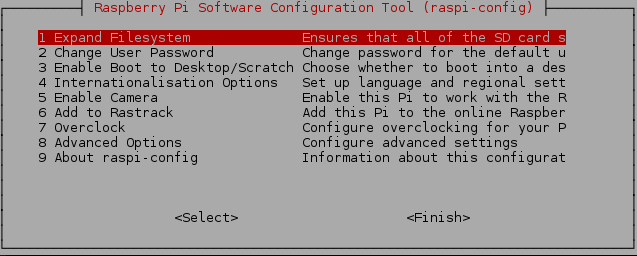
\includegraphics[scale=0.4]{2.png}
					\centering
					\caption{}
				\end{figure}
				\end{enumerate}
			\item Using Notepad++ and LXTerminal(or MobaXterm):
			      Notepad++ is a source code and a Windows text editor that is widely used by programmers.(It is more efficient than other text editors because it prompts you with indentation related errors that count in python programming) 
			\begin{enumerate}
				\item Open the application and a create a new file.
				\newpage
				\begin{figure}[h!]
					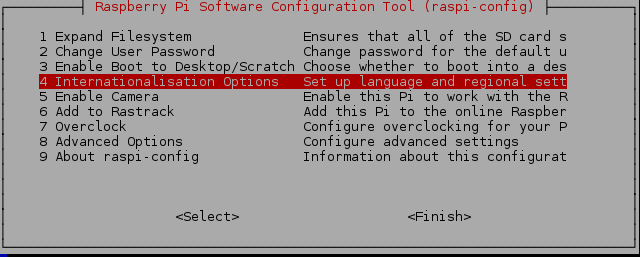
\includegraphics[scale=0.4]{3.png}
					\centering
					\caption{}
				\end{figure}
				\item Type your python code and then save it as filename.py 
				\item After that follow the steps(3-5) mentioned in the above method i.e using PScripter and MobaXterm.
			\end{enumerate}
			\item Using MobaXterm(for remote operation) or LXTerminal:
			In this method we can create a python file on the terminal window in the following way:
			\begin{enumerate}
				\item Open the MobaXterm or LXTerminal.
				\item Type the command \textit{touch filename.py} to create a file in a directory say home directory
				\item Once the file is created in order to edit it type the command \textit{nano filename.py}
				\newpage
				\begin{figure}[h!]
					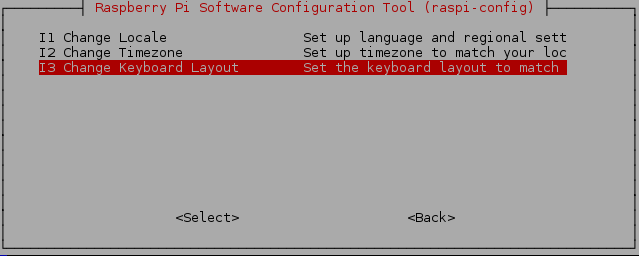
\includegraphics[scale=0.4]{4.png}
					\centering
					\caption{}
				\end{figure}
				\item A blank file opens as shown 
				\begin{figure}[h!]
					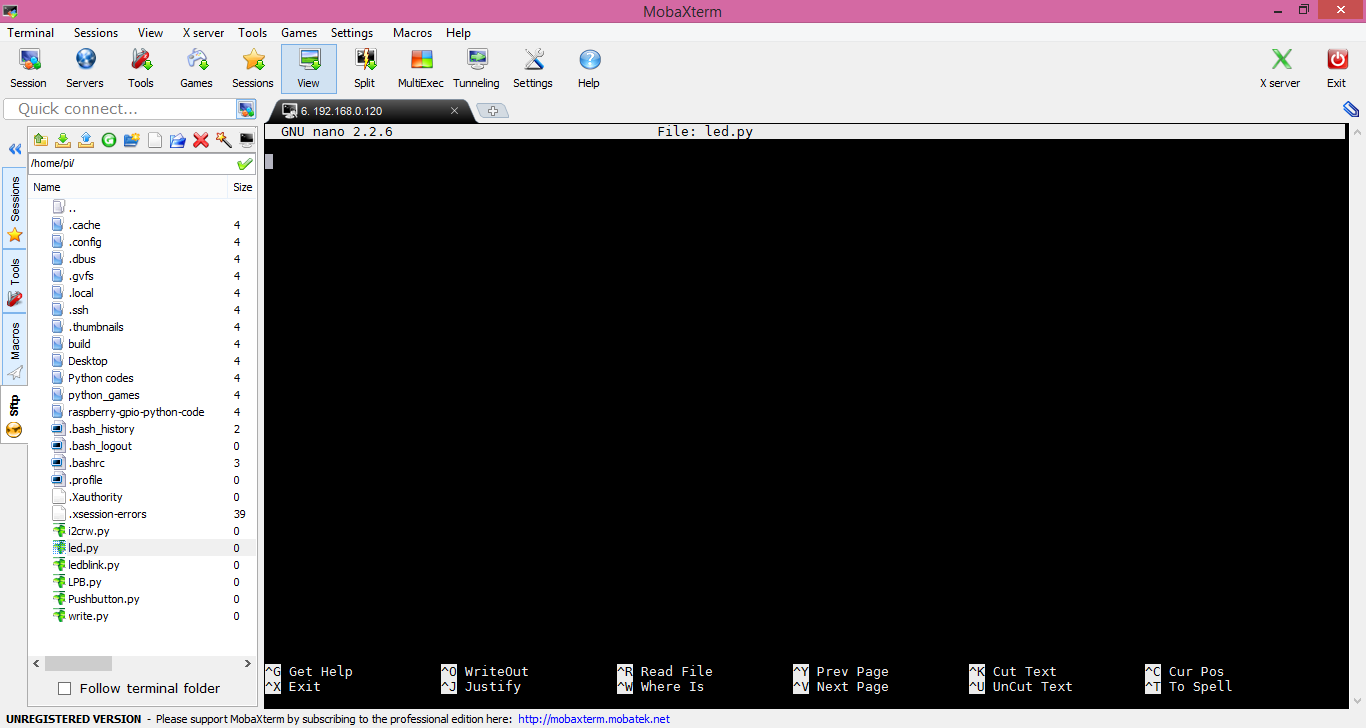
\includegraphics[scale=0.4]{5.png}
					\centering
					\caption{}
				\end{figure}
				\item Type the required code and save the contents by typing \textit{Ctrl + X,Y}(to save the file type Y)
				\item Then press enter to exit the editor onto terminal window.
				\item You can now execute the file by using the command \textit{sudo python filename.py}(Don't forget to change the directory if your file is not saved in the home directory.PLease refer the steps mentioned before in the document)
			\end{enumerate}
			Note: Just in case you want to view the contents of the file on the terminal window type \textit{cat filename.py}
		\end{itemize}				
	\end{enumerate}
	\vspace{0.3cm}
	Now we are all set to write basic programs to access GPIO pins in your R-Pi
	
	\newpage
	\section{Experiments}
	All codes of other experiments can be accessed through:- \url{abc.com}
	\subsection{Program to access GPIO pin of R-Pi for beeping Buzzer by push button}
	
		 \begin{itemize}
	 	\item Buzzer is connected to pin no. 4

	 	\item One pin of the push button is connected to Ground
	   	\item The other pin of the push button is connected to pin no. 18
	\end{itemize}

	\newpage
	\flushleft
	\textbf{Code:-}
	\vspace{0.3cm}
	\lstinputlisting[language=Python]{blink.py}
	\newpage
	\subsection{IR sensors  interfacing}
	The objective is to Interface the ADC MCP3008 to 8 IR sensors.ADC MCP3008 operates on SPI protocol. \vspace{0.2cm}\newline
	\textbf{Enabling SPI}\vspace{0.2cm}\newline
	Enabling using raspi-config\newline
	Run the following command:\newline
Sudo raspi-config\newline
This will launch the raspi-config utility. Select option 8 "Advanced Op-
tions".\newline
\begin{figure}[h!]
		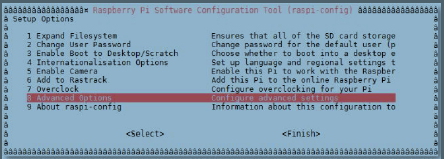
\includegraphics[scale=0.7]{spi1.png}
		\centering
		\caption{}
	    \end{figure}\newline
Select the "SPI" option.\newline
\begin{figure}[h!]
		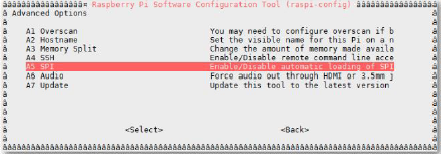
\includegraphics[scale=0.7]{spi2.png}
		\centering
		\caption{}
	    \end{figure}\newline
	    Set the option to "Yes".\newline
	   
Select "OK".\newline
 \newline
	   Select "Finish".\newline
	 \newline
	    Reboot for the changes to take effect :\newline
sudo reboot\newline
SPI is now enabled.\vspace{0.9cm}\newline
\textbf{Installing SPI Wraper in python }\vspace{0.2cm}\newline
In order to read data from the SPI bus in Python we can install a library
called `py-spidev'. To install it we first need to install `python-dev':
sudo apt-get install python2.7-dev
Then to finish we can download `py-spidev' and compile it ready for use,
run the following commands:
wget https://github.com/Gadgetoid/py-spidev/archive/master.zip
unzip master.zip
rm master.zip
cd py-spidev-master
sudo python setup.py install
cd ..
You should now be ready to either communicate with add-on boards us-
ing their own libraries (e.g. the PiFace) or other SPI devices.
	\vspace{0.2cm}
	\newline
	

	 \begin{figure}[h!]
		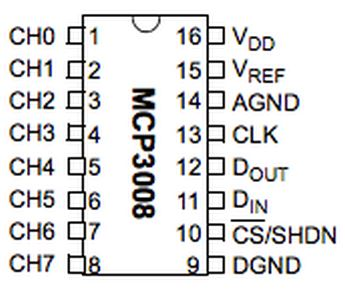
\includegraphics[scale=0.7]{mcp.jpg}
		\centering
		\caption{MCP3008 IC}
	    \end{figure}
	
	IR sensors are connected to ADC 1  to the specific channels as shown :-
		\vspace{0.3cm}
	
	\centering
	\begin{tabular}{ |p{3cm}|p{3cm}| }
	

 \hline
 IR sensor number& ADC channel\\
 \hline
 IR 1&0\\
 \hline
 IR 2&1\\
 \hline
 IR 3&2\\
 \hline
 IR 4&3\\
 \hline
 IR 5&4\\
 \hline
 IR 6&5\\
 \hline
 IR 7&6\\
 \hline
 IR 8&7\\
 \hline
\end{tabular}

		
	\newpage
	\flushleft
	\textbf{Code:-}
	\vspace{0.3cm}
	\lstinputlisting[language=Python]{adc.py}
	\newpage
	\subsection{LCD interface with port expander}
	In this tutorial we will be interfacing LCD with R-pi using port expander .MCP 23017 is based on I@C protocol.\newline
	
	\textbf{Enabling I2C}\vspace{0.2cm}\newline
	Enabling using raspi-config\newline
	Run the following command:\newline
Sudo raspi-config\newline
This will launch the raspi-config utility. Select option 8 "Advanced Op-
tions".\newline
\begin{figure}[h!]
		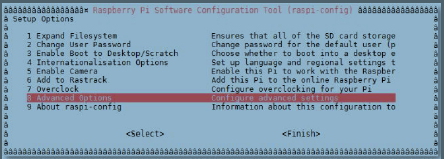
\includegraphics[scale=0.7]{spi1.png}
		\centering
		\caption{}
	    \end{figure}\newline
Select the "I2C" option.\newline
\begin{figure}[h!]
		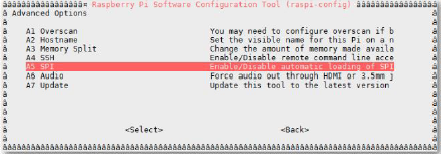
\includegraphics[scale=0.7]{spi2.png}
		\centering
		\caption{}
	    \end{figure}\newline
	    Set the option to "Yes".\newline
	   
Select "OK".\newline
 \newline
	   Select "Finish".\newline
	 \newline
	    Reboot for the changes to take effect :\newline
sudo reboot\newline
I2C is now enabled.\vspace{0.2cm}\newline
When you power up or reboot your Pi you can check the i2c module is running by using the following command : \newline \textit{lsmod | grep i2c\_} \newline That will list all the modules starting with “i2c\_”. If it lists “i2c\_bcm2708” then the module is running correctly.\newline
		 Once you have connected your hardware double check the wiring. Make sure 3.3V is going to the correct pins and you have got not short circuits. Power up the Pi and wait for it to boot.\newline
		Type the command: \newline \textit{sudo i2cdetect -y 1} \newline
		You should the output as:\newline
			\begin{figure}[h!]
				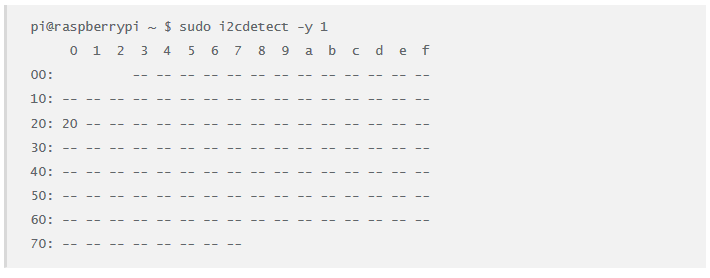
\includegraphics[scale=0.6]{i2c_9.png}
				\centering
				\caption{[4]}
			\end{figure}
			LCD is connected to portA of port expander 1 inthe order :-	
			vspace{0.3cm}
	
	\centering
	\begin{tabular}{ |p{3cm}|p{3cm}| }
	

 \hline
 LCD pin& port expander 1 port A pin\\
 \hline
 RS&pA0\\
 \hline
 EN pA1\\
 \hline
 D5&pA2\\
 \hline
 D4&pA3\\
 \hline
 D6&pA4\\
 \hline
 D7&pA5\\
 \hline

\end{tabular}
			\newpage
	\flushleft
	\textbf{Code:-}
	\vspace{0.3cm}
	\lstinputlisting[language=Python]{i2clcd.py}
	\newpage
	
	
	    \subsection{Xbee Communication}
	    
	    In this experiment we will study to enable the serial communication through XBEE.  \vspace{0.3cm}\newline
	     \textbf{Enabling Serial communication in Pi}\newline
	     Refer to link :- \href{https://electrosome.com/uart-raspberry-pi-python/}{Enabling Guide[10]}
	    \vspace{0.2cm} \newline
	    
	    \flushleft
	\textbf{Code:-}
	
	\lstinputlisting[language=Python]{xbee.py}
	\newpage
	\subsection{Servo motors}
	We have given 3 ports on adaptor board to control the 3 servo motors and their enable pins are connected to the following Raspberry-pi pins:-
	
	\centering
	\begin{tabular}{ |p{3cm}|p{3cm}| }

 \hline
 Servo motor& Raspberry pin(GPIO)\\
 \hline
 Servo1&18\\
 \hline
 Servo2&23\\
 \hline
 Servo3&24\\
 \hline
 \end{tabular}
 \vspace{0.2cm} 
	    \flushleft
	\textbf{Code:-}
	\lstinputlisting[language=Python]{servo.py}

	\newpage

	\subsection{Turning off pi with press of push button}
	In order to protect our SD card from getting corrupted we should shut down the Raspberry-Pi properly instead of powering it off directly.\\
	So in order to do that we have put a intterupt switch on the Adaptor Board .When we will press the switch the Raspberry pi will be Switched off or Shut Down properly .
	We are using a Pull up register for checking the Input,so if button is pressed then output will be 0 as we are using it in pull up configuration \\
	We have connected the interupt switch to GPIO 20 of raspberry pi.
	\vspace{0.2cm} \newline
	    \flushleft
	\textbf{Code:-}
	\lstinputlisting[language=Python]{shut.py}
	

	
		\newpage
	\chapter{References}
		\begin{enumerate}
		\item \url{https://www.raspberrypi.org/}
		\item \url{http://en.wikipedia.org/wiki/Raspberry_Pi}	
		\item \url{https://www.raspberrypi.org/wp-content/uploads/2014/11/Raspberry_Pi_Family_A-annotated-15001.jpg}
		\item \url{http://assets.windowsphone.com/3f82dfe6-a179-4ddf-9738-91989190c3fa/IoT-rpi2-board_InvariantCulture_Default.png}	
		\item \url{http://en.wikipedia.org/wiki/Secure_Shell}
		\item \url{http://www.webopedia.com/TERM/S/SSH.html}
		\item \url{http://www.codemastershawn.com/library/tutorial/images/ssh.tunnel.overview.gif}
		\item \url{http://mobaxterm.mobatek.net/}
		\item \url{http://www.suntimebox.com/raspberry-pi-tutorial-course/week-3/day-5/}
		\item \url{https://electrosome.com/uart-raspberry-pi-python/}
	\end{enumerate}
	
	
\end{flushleft}
\end{document}



